\documentclass[a4paper,11pt,twoside]{article}
\usepackage[T1]{fontenc}
\usepackage[utf8]{inputenc}
\usepackage{ngerman, eucal, mathrsfs, amsfonts, bbm, amsmath, amssymb, stmaryrd,graphicx, array, geometry, color, wrapfig}
\geometry{left=25mm, right=15mm, bottom=25mm}
\setlength{\parindent}{0em} 
\setlength{\headheight}{0em} 
\title{Machine Learning\\ Blatt 1}
\author{Markus Vieth, David Klopp, Christian Stricker}
\date{\today}
\usepackage{listings, textcomp}
\usepackage[usenames,dvipsnames,svgnames,table]{xcolor}


\definecolor{Code}{rgb}{0,0,0}
\definecolor{Keywords}{rgb}{0,0,255}
\definecolor{Strings}{rgb}{255,0,0}
\colorlet{Comments}{Green}
\colorlet{Numbers}{blue}

%%%%%%%%%%%
%Mache Integer farbig
%%%%%%%%%%%

\makeatletter

\newif\iffirstchar\firstchartrue
\newif\ifstartedbyadigit

\newcommand\processletter
{%
	\ifnum\lst@mode=\lst@Pmode%
	\iffirstchar%
	\global\startedbyadigitfalse%
	\fi
	\global\firstcharfalse%
	\fi
}

\newcommand\processdigit
{%
	\ifnum\lst@mode=\lst@Pmode%
	\iffirstchar%
	\global\startedbyadigittrue%
	\fi
	\global\firstcharfalse%
	\fi
}

\lst@AddToHook{Output}%
{%
	\ifstartedbyadigit%
	\def\lst@thestyle{\color{Numbers}}%
	\fi
	\global\firstchartrue%
	\global\startedbyadigitfalse%
}

\newtoks\jubo@toks
\jubo@toks={
	language=C,
	commentstyle=\color{Comments}\slshape,
	stringstyle=\color{Strings},
	keywordstyle={\color{Keywords}\bfseries},
	alsoletter=0123456789,
	SelectCharTable=%
}
\def\add@savedef#1#2{%
	\begingroup\lccode`?=#1\relax
	\lowercase{\endgroup
		\edef\@temp{%
			\noexpand\lst@DefSaveDef{\number#1}%
			\expandafter\noexpand\csname lsts@?\endcsname{%
				\expandafter\noexpand\csname lsts@?\endcsname\noexpand#2}%
		}}%
		\jubo@toks=\expandafter{\the\expandafter\jubo@toks\@temp}%
	}
	\count@=`0
	\loop
	\add@savedef\count@\processdigit
	\ifnum\count@<`9
	\advance\count@\@ne
	\repeat
	\count@=`A
	\loop
	\add@savedef\count@\processletter
	\ifnum\count@<`Z
	\advance\count@\@ne
	\repeat
	\count@=`a
	\loop
	\add@savedef\count@\processletter
	\ifnum\count@<`z
	\advance\count@\@ne
	\repeat
	%\showthe\jubo@toks % for debugging
	\begingroup\edef\x{\endgroup
		\noexpand\lstdefinestyle{pseudo}{\the\jubo@toks}
	}\x
	
	\makeatother
%%%%%%%%%%
%Ende
%%%%%%%%%%



\lstset{
	literate={ö}{{\"o}}1
	{ä}{{\"a}}1
	{ü}{{\"u}}1
	{ß}{{\ss}}1
	{/pi}{{$\Pi$}}1
	{/inf}{{$\infty$}}1
	{/eIn}{{$\in$}}1
	{/cup}{{$\cup$}}1
	{/leer}{{$\emptyset$}}1
	{<=}{{$\leq$}}1
	{>=}{{$\geq$}}1
}


\lstset{
	numberstyle=\tiny,
	stepnumber=1,
	numbersep=10pt,
	xleftmargin=15pt,
	breaklines=true,
	numberblanklines=false,
	showstringspaces=false,
	flexiblecolumns=true,
	mathescape=true,
	tabsize=4,
	captionpos=b,
	numbers=left,
	commentstyle=\color{Green},
	numberstyle=\color{gray},
	keywordstyle=\color{blue} \textbf,%otherkeywords={xdata},
	keywords=[2]{xdata},
	keywordstyle=[2]\color{red}\textbf,
	identifierstyle=\color{black},
	stringstyle=\color{red}\ttfamily,
	basicstyle = \ttfamily \color{black} \footnotesize,
	inputencoding=utf8,
	emph=[1]%
	{%
		infinity,
	}, 
	emphstyle=[1]{\color{blue}},
	emph=[2]%
	{%
		forall,
		while,
		if,
		else,
		for,
		return,
		new,
		NULL,
		null,
		int, 
		double, 
		float,
		class,
		void,
		false, 
		true,
		FALSE,
		TRUE,
	}, 
	emphstyle=[2]{\color{Magenta}},
	emph=[3]{b0, b1, n0, n1},
	emphstyle=[3]{\color{black}}
}
\begin{document}

\newcommand{\cor}[1]{\textcolor{red}{\textit{#1}}}
\maketitle
\cleardoublepage
\pagestyle{myheadings}
\markboth{Markus Vieth,  David Klopp, Christian Stricker}{Markus Vieth, David Klopp, Christian Stricker}

\section*{Nr.1}

\subsection*{a)}
\begin{wrapfigure}[18]{l}{0.3\linewidth}
	\begin{center}
		\vspace*{-3em}
		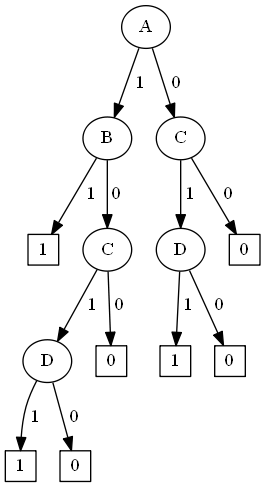
\includegraphics[width=\linewidth]{Aufgabe1/graphA.png}
	\end{center}
\end{wrapfigure}
$~$\\
$~$\\
$~$\\
$~$\\
$~$\\
$~$\\
$~$\\
$~$\\
$~$\\
$~$\\
$~$\\
$~$\\
$~$\\
$~$\\
$~$\\
$~$\\
$~$\\
$~$\\
$~$\\
$~$\\
\subsection*{b)}
\begin{wrapfigure}[7]{l}{0.5\textwidth}
	\begin{center}
		
		\vspace*{-3em}
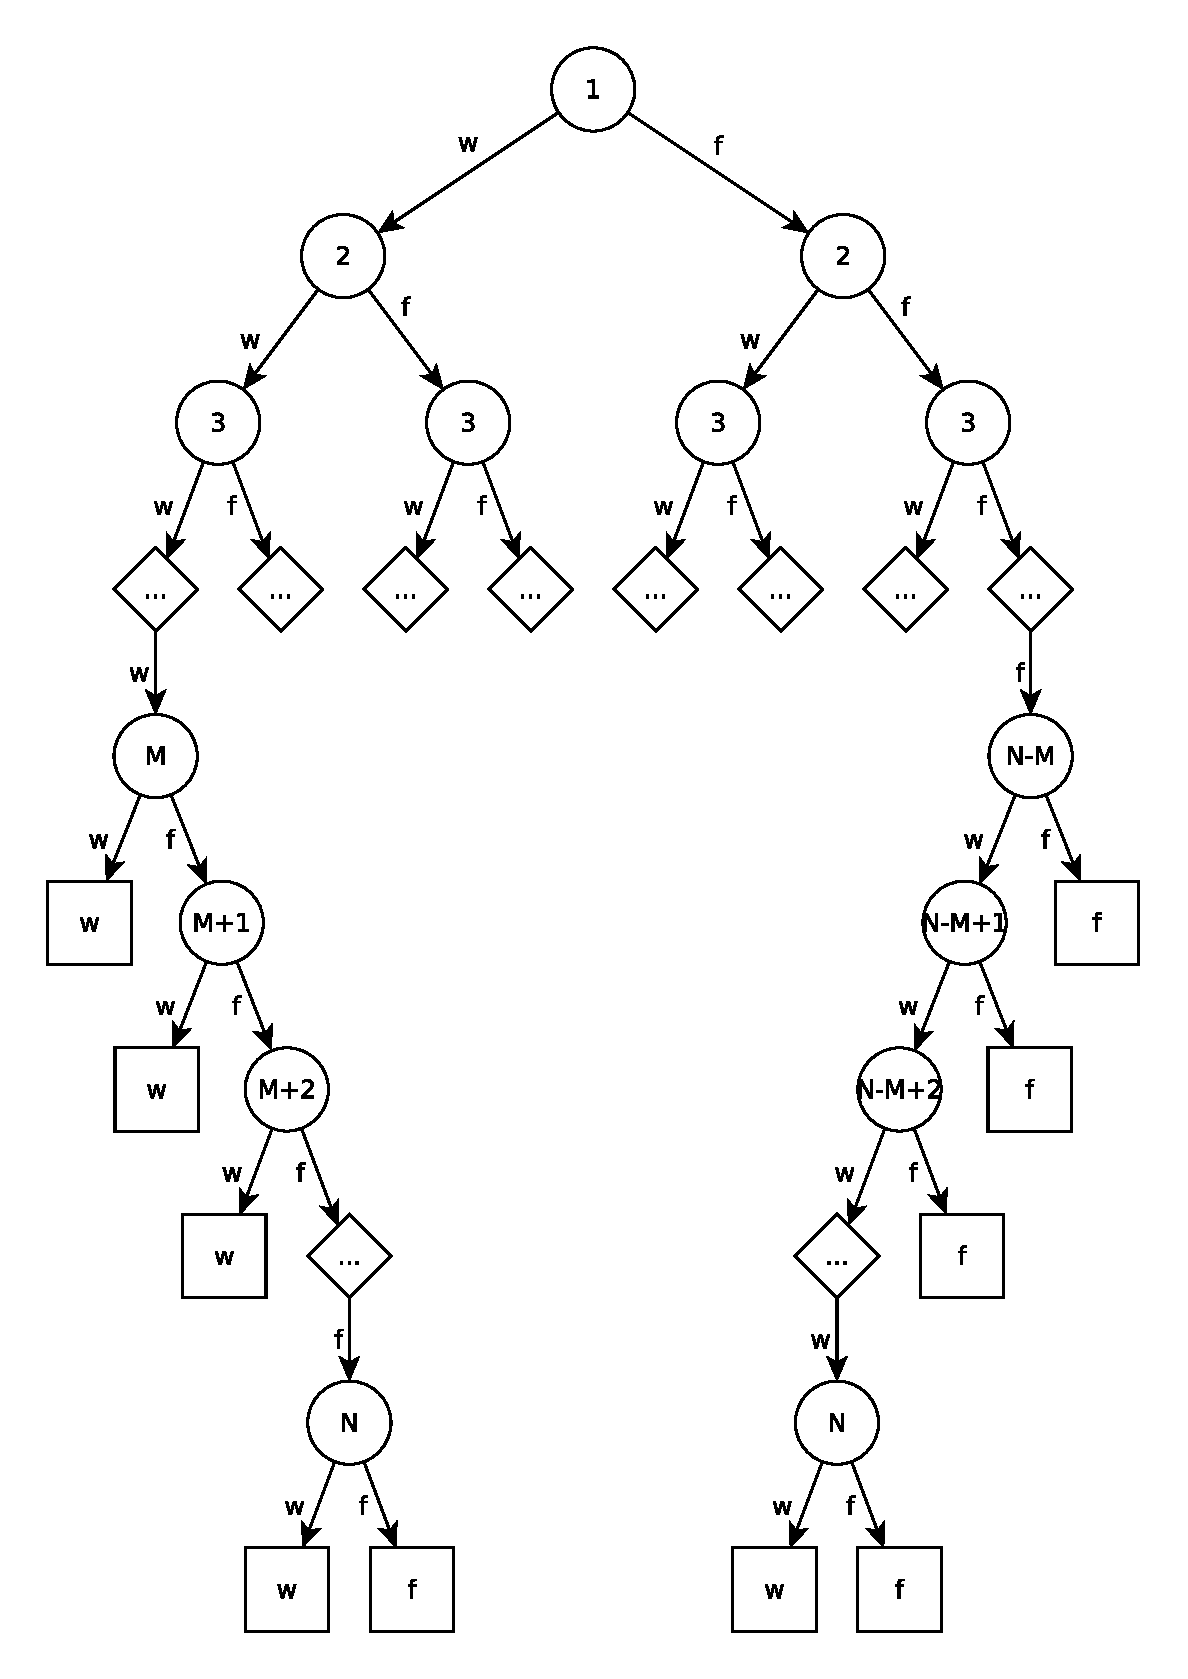
\includegraphics[width=\linewidth]{Aufgabe1/graphB.eps}
\end{center}
\end{wrapfigure}
Skizze des M-von-N-Baumes. Die Teilbäume der Knoten M bis N und N-M bis N finden sich (teilweise verkürzt) in der Mitte des Baumes wieder. Der Baum hat eine maximale Tiefe von N und eine maximale Breite von $2^{M+1}$ im Level $M+1$ \cor{Leichter ist es den Baum formal zu beschreiben (wie ein Programm). So bleibt einiges offen. -0,5}
\newpage

\section*{Nr.3}
\subsection*{a)}
$S = \{A,B,C,D\}$ 
\[ H(S) = -p(A)log2(p(A))-p(B)log2(p(B))-p(C)log2(p(C))-p(D)log2(p(D)) \]
\[ = -0,5*log2(0,5)-0,3*log2(0,3)-0,1*log2(0,1)-0,1*log2(0,1) \]
\[ = 1.685475297227334319499038031560350135304471374204545987890...\]

\subsection*{b)}
$max = log2(|S|)~~,\forall x \in S ~~~\text{gilt:}~~~ p(x) = 1/|S|$\\
$min = 0 \Leftrightarrow \exists x \in S ~~~\text{mit}~~~ p(x) = 1  \Rightarrow \forall y \in S \setminus \{x\} : p(y) = 0$

\subsection*{c)}
Entropie ist eine Skala für die Verteilung der Werte des Klassenattributes auf die Werte des betrachteten Attributes. Somit bedeutet eine niedrige Entropie, dass sich die Werte des Klassenattributes auf einige wenige Werte des betrachteten Attributes verteilen, wo hingegen eine hohe Entropie bedeutet, dass sich die Werte des Klassenattributes gleichmäßig auf die Werte des betrachteten Attributes verteilen.
\paragraph{Kodierung}
\begin{tabular}{cc}
	Symbol & Code-Wort \\
	A & 0\\
	B & 10\\
	C & 110\\
	D & 111
\end{tabular}

\subsection*{d)}
Bei einem Entscheidungsbaum ist die Reihenfolge der Betrachtung der Attribute für dessen Komplexität von Bedeutung. Die Qualität \cor{naja} eines Attributes kann mithilfe des InformationGains bewertet werden. Dazu betrachten wir die erwartete Verminderung der aktuellen Entropie bei Wahl des betrachteten Attributes. Durch eine niedrige erwartete Entropie wird der Baum kürzer. \cor{Wie wird das gemacht? -1,5}


\section*{Nr.5}
\paragraph{Anmerkung}
Es wurden im Prinzip die Klassen aus der bereitgestellten .jar verwendet. Es wurden jedoch 2 Änderungen vorgenommen.
\begin{enumerate}
	\item Ein Dataset kennt seinen ClassIndex
	\item Ein Attribute weiß, welchen Typ es hat
\end{enumerate}
\pagebreak
\subsection*{Code}
\lstinputlisting[language = java]{Aufgabe5/src/DecisionTree.java}


\end{document}